%%%%%%%%%%%%%%%%%%%%%%%%%%%%%%%%%%%%%%%%%%%%%%%%%%%
\documentclass[graybox]{svmult}
% choose options for [] as required from the list  in the Reference Guide
\usepackage{mathptmx}       % selects Times Roman as basic font
\usepackage{helvet}         % selects Helvetica as sans-serif font
\usepackage{courier}        % selects Courier as typewriter font
%\usepackage{type1cm}        % activate if the above 3 fonts are not available on your system
\usepackage{makeidx}         % allows index generation
\usepackage{graphicx}        % standard LaTeX graphics tool
\usepackage{multicol}        % used for the two-column index
\usepackage[bottom]{footmisc}% places footnotes at page bottom
\usepackage{amsmath,amssymb,amsfonts}        % AMS math packages
% see the list of further useful packages in the Reference Guide
\makeindex             % used for the subject index
% please use the style svind.ist with your makeindex program

%%%%%%%%%%%%%%%%%%%%%%%%%%%%%%%%%%%%%%%%%%%%%%%%%%%%%%%%%%%%%%%%%%%%
\begin{document}
\title*{Contribution Title}
% Use \titlerunning{Short Title} for an abbreviated version of
% your contribution title if the original one is too long
\author{Name of First Author and Name of Second Author}
% Use \authorrunning{Short Title} for an abbreviated version of
% your contribution title if the original one is too long
\institute{Name of First Author \at Name, Address of Institute, \email{name@email.address}
\and Name of Second Author \at Name, Address of Institute \email{name@email.address}}
%
% Use the package "url.sty" to avoid
% problems with special characters
% used in your e-mail or web address
%
\maketitle

\abstract{Each article should be preceded by an abstract (10--15 lines long) that summarizes the content. 
The abstract will appear online at \url{www.SpringerLink.com}.\newline\indent
Abstracts may have more than one paragraph.
}

\section{Section Heading}
\label{sec:1}
Every heading should be followed by at least a short passage of text. The first line of text that follows a heading is not indented, whereas the first lines of all subsequent paragraphs are. Use the \LaTeX\ \verb!label! and \verb!ref! commands for cross-references and citations. 

\section{Section Heading}
\label{sec:2}
% Always give a unique label
% and use \ref{<label>} for cross-references
% and \cite{<label>} for bibliographic references
% use \sectionmark{}
% to alter or adjust the section heading in the running head

Use the standard \verb|equation| environment to typeset your equations, e.g.
%
\begin{equation}
a \times b = c\;,
\end{equation}
%
and for multiline equations use the amsmath \verb|align| environment:
\begin{align}
a \times b & = c \nonumber\\
\vec{a} \cdot \vec{b} & =\vec{c}
\label{eq:01}
\end{align}

\subsection{Subsection Heading}
\label{subsec:2}

Please use the \LaTeX\ automatism for all your
cross-references\index{cross-references} and citations\index{citations}
as has already been described in Sect.~\ref{sec:2}.

\begin{quotation}
Please do not use quotation marks when quoting texts. Simply use the \verb|quotation| environment -- it will automatically render Springer's preferred layout.
\end{quotation}


\subsubsection{Subsubsection Heading}

See Fig.~\ref{fig:1} for an example showing how to typeset a figure\footnote{If you copy
text passages, figures, or tables from other works, you must obtain
\textit{permission} from the copyright holder (usually the original
publisher). Please enclose the signed permission with the manuscript. The
sources\index{permission to print} must be acknowledged.}

% For figures use
%
\begin{figure}[b]
\sidecaption
% Use the relevant command for your figure-insertion program
% to insert the figure file.
% For example, with the graphicx style use
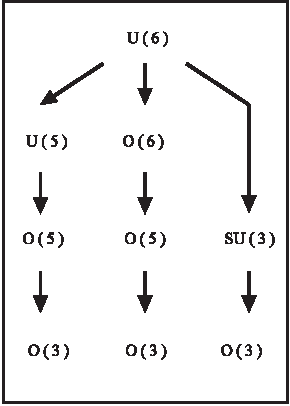
\includegraphics[scale=.65]{figure}
%
% If no graphics program available, insert a blank space i.e. use
%\picplace{5cm}{2cm} % Give the correct figure height and width in cm
%
\caption{If the width of the figure is less than 7.8 cm use the \texttt{sidecapion} command to flush the caption on the left side of the page. If the figure is positioned at the top of the page, align the sidecaption with the top of the figure -- to achieve this you simply need to use the optional argument \texttt{[t]} with the \texttt{sidecaption} command}
\label{fig:1}       % Give a unique label
\end{figure}


\paragraph{Paragraph Heading} %

For typesetting numbered lists use the \verb|enumerate| environment. For unnumbered list use the \verb|itemize| environment. They will automatically render Springer's preferred layout.

\begin{enumerate}
\item{Livelihood and survival mobility are often outcomes of uneven socioeconomic development.}
\begin{enumerate}
\item{Livelihood and survival mobility are often outcomes of uneven socioeconomic development.}
\item{Livelihood and survival mobility are often outcomes of uneven socioeconomic development.}
\end{enumerate}
\item{Livelihood and survival mobility are often times coutcomes of uneven socioeconomic development.}
\end{enumerate}


\subparagraph{Subparagraph Heading} 

\begin{figure}[t]
\sidecaption[t]
% Use the relevant command for your figure-insertion program
% to insert the figure file.
% For example, with the option graphics use
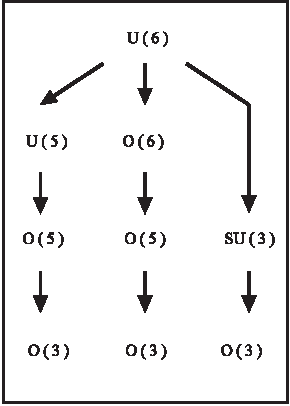
\includegraphics[scale=.65]{figure}
\caption{If the width of the figure is less than 7.8 cm use the \texttt{sidecapion} command to flush the caption on the left side of the page. If the figure is positioned at the top of the page, align the sidecaption with the top of the figure -- to achieve this you simply need to use the optional argument \texttt{[t]} with the \texttt{sidecaption} command}
\label{fig:2}       % Give a unique label
\end{figure}

\runinhead{Run-in Heading Boldface Version} Use  \LaTeX\ cross-references and citations as has already been described in Sect.~\ref{sec:2}.

\subruninhead{Run-in Heading Italic Version} Format tables as shown in Table~\ref{tab:1}.

% Use the \index{} command to code your index words
%
% For tables use
%
\begin{table}
\caption{Please write your table caption here}
\label{tab:1}       % Give a unique label
%
% Follow this input for your own table layout
%
\begin{tabular}{p{2cm}p{2.4cm}p{2cm}p{4.9cm}}
\hline\noalign{\smallskip}
Classes & Subclass & Length & Action Mechanism  \\
\noalign{\smallskip}\svhline\noalign{\smallskip}
Translation & mRNA$^a$  & 22 (19--25) & Translation repression, mRNA cleavage\\
Translation & mRNA cleavage & 21 & mRNA cleavage\\
Translation & mRNA  & 21--22 & mRNA cleavage\\
Translation & mRNA  & 24--26 & Histone and DNA Modification\\
\noalign{\smallskip}\hline\noalign{\smallskip}
\end{tabular}
$^a$ Table foot note (with superscript)
\end{table}
%

\subsection{Subsection Heading}
\label{sec:3}

For definitions and the like use the Springer-enhanced \verb|description| environment.

\begin{description}[Type 1]
\item[Type 1]{That addresses central themes pertainng to migration, health, and disease. In Sect.~\ref{sec:1}, Wilson discusses the role of human migration in infectious disease distributions and patterns.}
\item[Type 2]{That addresses central themes pertainng to migration, health, and disease. In Sect.~\ref{subsec:2}, Wilson discusses the role of human migration in infectious disease distributions and patterns.}
\end{description}

\begin{svgraybox}
To emphasize complete paragraphs of texts use the Springer class option \verb|graybox| and the environment \verb|svgraybox|. This will produce a 15 percent screened box 'behind' your text.
\end{svgraybox}


\subsubsection{Subsubsection Heading}

\begin{theorem}
Theorem text goes here.
\end{theorem}

\begin{theorem}[Four-Colour Theorem \cite{science-DOI}] 
Theorem text goes here.
\end{theorem}
%
% or
%
\begin{definition}
Definition text goes here.
\end{definition}

\begin{proof}
%\smartqed
Proof text goes here.
\qed
\end{proof}

%
\begin{acknowledgement}
If you want to include acknowledgments please use the \verb|acknowledgement| environment -- it will automatically render Springer's preferred layout.
\end{acknowledgement}
%

Please do not use an appendix.

\bigskip
%
% BibTeX users please use
% \bibliographystyle{spmpsci}
% \bibliography{}
%
References should be cited in the text by number (rather than author/year). All references should be cited in the text. The reference list should be sorted in alphabetical order. If there are several works by the same author, the following order should be used: 
\begin{enumerate}
\item all works by the author alone, ordered chronologically by year of publication
\item all works by the author with a coauthor, ordered alphabetically by coauthor
\item all works by the author with several coauthors, ordered chronologically by year of publication.
\end{enumerate}
Use the BibTeX bibliography style file \texttt{spmpsci.bst}, or follow the examples below. Use the standard abbreviation of a journal's name according to the ISSN List of Title Word Abbreviations (\url{http://www.issn.org/}).

\begin{thebibliography}{99.}%
% and use \bibitem to create references.
%
% Use the following syntax and markup for your references if 
% the subject of your book is from the field 
% "Mathematics, Physics, Statistics, Computer Science"
%
% Contribution 
\bibitem{science-contrib} Broy, M.: Software engineering --- from auxiliary to key technologies. In: Broy, M., Dener, E. (eds.) Software Pioneers, pp. 10-13. Springer, Heidelberg (2002)
%
% Online Document
\bibitem{science-online} Dod, J.: Effective substances. In: The Dictionary of Substances and Their Effects. Royal Society of Chemistry (1999) Available via DIALOG. \\
\url{http://www.rsc.org/dose/title of subordinate document. Cited 15 Jan 1999}
%
% Monograph
\bibitem{science-mono} Geddes, K.O., Czapor, S.R., Labahn, G.: Algorithms for Computer Algebra. Kluwer, Boston (1992) 
%
% Journal article
\bibitem{science-journal} Hamburger, C.: Quasimonotonicity, regularity and duality for nonlinear systems of partial differential equations. Ann. Mat. Pura. Appl. \textbf{169}, 321--354 (1995)
%
% Journal article by DOI
\bibitem{science-DOI} Slifka, M.K., Whitton, J.L.: Clinical implications of dysregulated cytokine production. J. Mol. Med. (2000) doi: 10.1007/s001090000086 
%
\end{thebibliography}
\end{document}
